% ----------------------------------------------------------
\chapter{Systematic Review of the Literature: AI, ML and Law} \label{ap:rsl_ml_law}
% ----------------------------------------------------------

The Systematic Review of the Literature, detailed in this section, focused on finding works related to the applications of TM and ML in the legal domain.


\section{Definition of Search Questions}

The main question in this SRL is: ``Which are the Text Mining Techniques applied in the legal domain?''

As secondary questions, there is:

\begin{itemize}[noitemsep]
    \item Which is the legal application?
    \item What are the pre-processing techniques used?
    \item What are the representation techniques used?
    \item What are the feature extraction techniques used?
    \item What are the classification techniques used?
    \item What are the clustering techniques used?
    \item What are the regression techniques used?
    \item What are the evaluation techniques used?
\end{itemize}

\section{Search Strategies}

In order to have an overview of the publications regarding TM and legal domain, we searched in February 29, 2020, for works published on conferences or journals from 2010 to 2020.  The search used the following search string:

\begin{verbatim}
    ("text mining" OR "natural language processing" OR "nlp" OR
    "language processing") AND ("deep learning" OR "machine learning")
    AND ("classification" OR "cluster*" OR "regression" OR 
    "categorization" OR "embedding*" OR "representation" OR "predict*")
    AND ("text" OR "document") AND ("law" OR "legal" OR "judicial" OR
    "justice" OR "court" OR "legislation" OR "juridical" OR "lawful")
\end{verbatim}

In this search, we also added synonymous for Machine Learning, Text Mining, and ML Tasks, and the legal domain.

The search embraced the papers' titles, abstracts and keywords.

\section{Knowledge Bases}

In this SRL, we included bases predominantly related to computing as well as interdisciplinary basis.  The list of knowledge bases follows:

\begin{itemize}[noitemsep]
    \item Scopus
    \item IEEE Xplore
    \item Web of Science
    \item ACM Digital Library
\end{itemize}

\section{Inclusion and Exclusion Criteria}

Following the questions of this research, we defined a set of inclusion and exclusion criteria. The process of selection embraced the reading of title, abstract and keywords and the accordance with the criteria:

The following is the list of inclusion criteria:

\begin{itemize}[noitemsep]
    \item Published in journal or conference
    \item Involves legal processes, or texts with juridical language;
    \item Involves Machine Learning or Text Mining;
    \item The techniques used are named;
    \item Empirical Works.
    \item Published from 2010 and February 2020.
\end{itemize}

And the following is the list of exclusion criteria:

\begin{itemize}[noitemsep]
    \item Not written in Portuguese or English;
    \item Published over 10 years ago;
    \item Does not involve Machine Learning or Text Mining;
    \item Does not involve the legal domain;
    \item Theoretical works.
\end{itemize}


\section{Data Extraction Plan}

Information to extract from the papers:

\begin{itemize}[noitemsep]
    \item Title
    \item Keywords
    \item Abstract
    \item Authors
    \item Year of publication
    \item Journal or Conference
    \item Authors affiliation
    \item Pre-processing techniques
    \item Representation / Feature Extraction Techniques
    \item Classification  / Clustering / Regression Techniques
    \item Other techniques
    \item Model Evaluation Techniques
\end{itemize}


\section{Search Execution and Preliminary Analysis}

After applying the search strings to the knowledge bases on February 29, 2020 without filters on year of publication, we obtained the number of publications shown in Figure \ref{fig:ap_rsl_tm_law}.

\begin{figure}[H]
    \centering
    \caption{Publications on ML and TM applied to the legal domain without year filtering}
    \label{fig:ap_rsl_tm_law}
    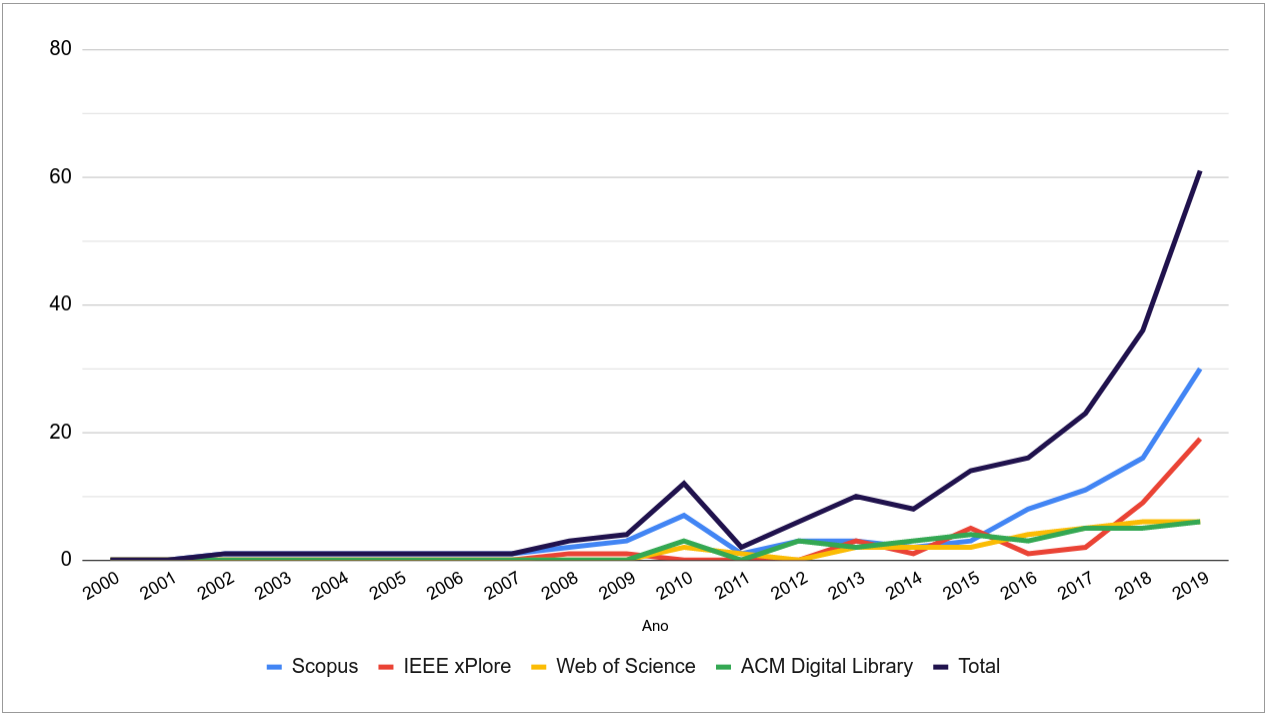
\includegraphics[width=\textwidth]{images/appendix/artigos_tm_law.png}
\end{figure}

After applying the search strings to the knowledge bases with time filtering on February 29, 2020, the search returned 195. After duplicates removal, the number of works reduced to 147. Finally, from the reading of title, abstract and keywords and the application of the selection criteria, the number of works selected for full reading reduced to 46.

The selected works were used as references in the Introduction chapter, in the Related Works and in the Background.

\section{Results and Analysis}
In this section we show a sequence of quantitative data in terms of the tens most frequent authors, journals, text mining techniques and others.

In the following tables, there is ten most frequent authors and conferences found in the SRL and the most frequent techniques for pre-processing, representation, classification, clustering and evaluation.

% Legal Applications?

% Authors

\begin{table}[H]
    \centering
    \caption{Ten most frequent authors}
    \label{tab:rsl_freq_authors}
    \begin{tabular}{@{}cc@{}}
    
    \toprule
    \textbf{Authors}     & \textbf{Papers} \\ \midrule
    Matthes, Florian     & 5               \\
    Glaser, Ingo         & 4               \\
    Chalkidis, Ilias     & 3               \\
    Scepankova, Elena    & 3               \\
    Quaresma, Paulo      & 2               \\
    Gonçalves, Teresa    & 2               \\
    Galgani, Filippo     & 2               \\
    Compton, Paul        & 2               \\
    Hoffmann, Achim      & 2               \\
    Androutsopoulos, Ion & 2               \\ \bottomrule
    
    \end{tabular}
\end{table}

% Journals / Conferences

\begin{table}[H]
    \centering
    \caption{Ten most frequent journals and conferences}
    \label{tab:rsl_freq_conferences}
\begin{tabular}{@{}p{14cm}c@{}}
\toprule
\multicolumn{1}{c}{\textbf{Journal / Conference}}                                                         & \textbf{Papers} \\ \midrule
Lecture Notes in Computer Science                                                                         & 8               \\
CEUR Workshop Proceedings                                                                                 & 4               \\
Frontiers in Artificial Intelligence and Applications                                                     & 3               \\
Artificial Intelligence and Law                                                                           & 2               \\
2010 6th International Conference on Wireless Communications, Networking and Mobile Computing, WiCOM 2010 & 1               \\
Proceedings of the ACM Conference on Computer and Communications Security                                 & 1               \\
Foundations and Trends in Information Retrieval                                                           & 1               \\
Conference on Legal Knowledge and Information Systems                                                     & 1               \\
Expert Systems with Applications                                                                          & 1               \\
International Conference on Cloud Computing and Services Science                                          & 1               \\ \bottomrule
\end{tabular}
\end{table}

% Pré-processing Techniques


\begin{table}[H]
\centering
\caption{Ten most frequent pre-processing techniques}
\label{tab:rsl_freq_pre_processing}

    \begin{tabular}{@{}ll@{}}
    
    \toprule
    \multicolumn{1}{c}{\textbf{Preprocessing}} & \multicolumn{1}{c}{\textbf{Papers}} \\ \midrule
    Stop words removal                         & 15                                  \\
    Lemmatization                              & 8                                   \\
    Stemming                                   & 7                                   \\
    Tokenization                               & 4                                   \\
    Lowercase                                  & 4                                   \\
    POS Tagging                                & 3                                   \\
    Normalization                              & 3                                   \\
    Remove punctuation                         & 3                                   \\
    Remove noise                               & 1                                   \\
    Regularization                             & 1                                   \\ \bottomrule
    
    \end{tabular}
\end{table}


% Representation Techniques
\begin{table}[H]
\centering
\caption{Ten most frequent representation techniques}
\label{tab:rsl_freq_representation}
\begin{tabular}{@{}lc@{}}
\toprule
\textbf{Representation}  & \textbf{Papers} \\ \midrule
TF-IDF                   & 19              \\
Word2Vec                 & 14              \\
Bag of Words             & 10              \\
N-Gram                   & 7               \\
Part-of-Speech Tag       & 6               \\
Named Entity Recognition & 5               \\
Doc2Vec                  & 4               \\
Word Embeddings          & 3               \\
FastText                 & 3               \\ 
BERT                     & 2               \\ \bottomrule
\end{tabular}
\end{table}

% Classification techniques
\begin{table}[H]
\centering
\caption{Ten most frequent classification techniques}
\label{tab:rsl_freq_classification}
\begin{tabular}{@{}cc@{}}
\toprule
\textbf{Classification Tech} & \textbf{Papers} \\ \midrule
Support Vector Machine       & 24              \\
Convolution Neural Network   & 19              \\
Naïve Bayes                  & 18              \\
Decision Tree                & 17              \\
k Nearest Neighbors          & 14              \\
Recurrent neural network     & 14              \\
Random Forest                & 13              \\
Long Short Term Memor y      & 13              \\
Logistic Regression          & 11              \\
Conditional Random Field     & 7               \\ \bottomrule
\end{tabular}
\end{table}


% Clustering Techniques
\begin{table}[H]
\centering
\caption{Most frequent clustering techniques}
\label{tab:rsl_freq_clustering}
\begin{tabular}{cc}
\hline
\textbf{Clustering Tech} & \textbf{Papers} \\ \hline
Hierarchical Clustering  & 2               \\
Fuzzy C-Means            & 1               \\
Hierarchical LDA         & 1               \\
k-Means                  & 1              
\end{tabular}
\end{table}

\begin{table}[H]
\centering
\caption{Ten most frequent Evaluation Metrics}
\label{tab:rsl_freq_evaluation}
\begin{tabular}{cc}
\hline
\textbf{Evaluation Metric} & \textbf{Papers} \\ \hline
F1-score                   & 23              \\
Accuracy                   & 21              \\
Precision                  & 20              \\
Recall                     & 19              \\
Cross-validation           & 6               \\
Rouge                      & 2               \\
Area under curve ROC       & 2               \\
ROC                        & 1               \\
BLEU                       & 1               \\ \hline
\end{tabular}
\end{table}



% Regression Techniques
This SRL did not find works that applied regression techniques in the legal domain.




